\documentclass{article}

\usepackage[english, russian]{babel}
\usepackage{amsmath}
\newcommand{\Mod}[1]{\ (\mathrm{mod}\ #1)}
\usepackage[letterpaper,top=2cm,bottom=2cm,left=3cm,right=3cm,marginparwidth=1.75cm]{geometry}
\usepackage[usenames,dvipsnames]{color}
\usepackage{caption}

\setlength{\abovedisplayskip}{3pt}
\setlength{\abovedisplayshortskip}{3pt}
\setlength{\belowdisplayskip}{3pt}
\setlength{\belowdisplayshortskip}{3pt}
\usepackage[14pt]{extsizes} 

\DeclareMathAlphabet{\pazocal}{OMS}{zplm}{m}{n}
\newcommand{\unif}{\pazocal{U}}

\linespread{1.6}

\usepackage{amsmath}
\usepackage{graphicx}
\usepackage[colorlinks=true, allcolors=blue]{hyperref}
\usepackage{fancyvrb} % for "\Verb" macro
\VerbatimFootnotes    % enable use of \Verb in footnotes

\title{Наблюдаемые и контролируемые параметры}
\date{}
\begin{document}
\maketitle

\section*{Данные таблицы}
Таблица datacenter.DC\_log представляет собой хранилище данных, в котором сохраняются результаты мониторинга и управления системой ЦОД. Каждая запись в этой таблице содержит информацию о текущем состоянии системы, включая данные о температуре, влажности, энергопотреблении и других параметрах. Эти данные позволят анализировать работу ЦОД. Ниже представленны столбцы этой таблицы и их описания.


\begin{itemize}
    \item \textbf{timestamp}: Дата и время записи.
    \item \textbf{cooling\_setpoint}: Уставка системы охлаждения.
    \item \textbf{humidity\_setpoint}: Уставка контроля влажности.
    \item \textbf{ahu\_supply\_temp}: Температура поставки воздуха оборудования AHU.
    \item \textbf{facility\_total\_electricity\_demand\_rate}: Общее электропотребление всего ЦОД.
    \item \textbf{air\_system\_total\_cooling\_energy}: Энергопотребление системы охлаждения.
    \item \textbf{temp\_z\_1 -- temp\_z\_11}: Температуры в разных зонах ЦОД (от первой (Z\_1) до последней (Z\_11)).
    \item \textbf{co2\_z\_1, co2\_z\_6, co2\_z\_11}: Уровень CO\textsubscript{2} в первом, центральном и последнем коридорах ЦОД.
    \item \textbf{rh\_z\_1, rh\_z\_6, rh\_z\_11}: Относительная влажность в первом, центральном и последнем коридорах ЦОД.
    \item \textbf{outdoor\_air\_drybulb\_temperature}: Температура наружного воздуха по сухому термометру.
    \item \textbf{outdoor\_air\_wetbulb\_temperature}: Температура наружного воздуха по влажному термометру.
    \item \textbf{outdoor\_air\_relative\_humidity}: Относительная влажность наружного воздуха.
    \item \textbf{wind\_speed}: Скорость ветра.
    \item \textbf{wind\_direction}: Направление ветра.
    \item \textbf{thermal\_zone\_supply\_plenum}: Температура воздуха внутри фальшпола.
\end{itemize}

Столбец timestamp типа DateTime, остальные столбца типа Float32.

\section*{Что агент контролирует?}

 RL-агент принимает решения относительно трех параметров: уставки включения системы охлаждения (cooling\_setpoint), температуры поставки воздуха AHU (ahu\_supply\_temp), и уставки контроля влажности (humidity\_setpoint). На основе наблюдений он выдает 3 нормализованных значения в дипазоне $[-1, 1]$. Затем эти значения пересчитываются в фактические диапазоны: $[15, 32]$ (°C) для уставки системы охлаждения; $[1, 99]$ (\%) для уставки контроля влажности; $[4, 16]$  (°C) для температуры поставки воздуха AHU.
 
\section*{Дэшборд}
Дэшборд предназначен для мониторинга состояния среды внутри ЦОД. Дэшборд предоставляет пользователям информацию о температуре, влажности, уровне CO\textsubscript{2} и энергопотреблении в реальном времени. Нижней границей каждого графика является минимальное значение за отображаемый период, а не ноль. Так сделано, чтобы можно было увидеть более мелкие колебания графиков.

Дэшборд состоит из следующих секций:

\begin{itemize}
\item {\textbf{Секция Температур.} (Рис. 1). В этой секции пользователю отображаются средние значения температур за последнюю минуту для каждого коридора ЦОД.

\begin{figure}[hbt!]
\centering
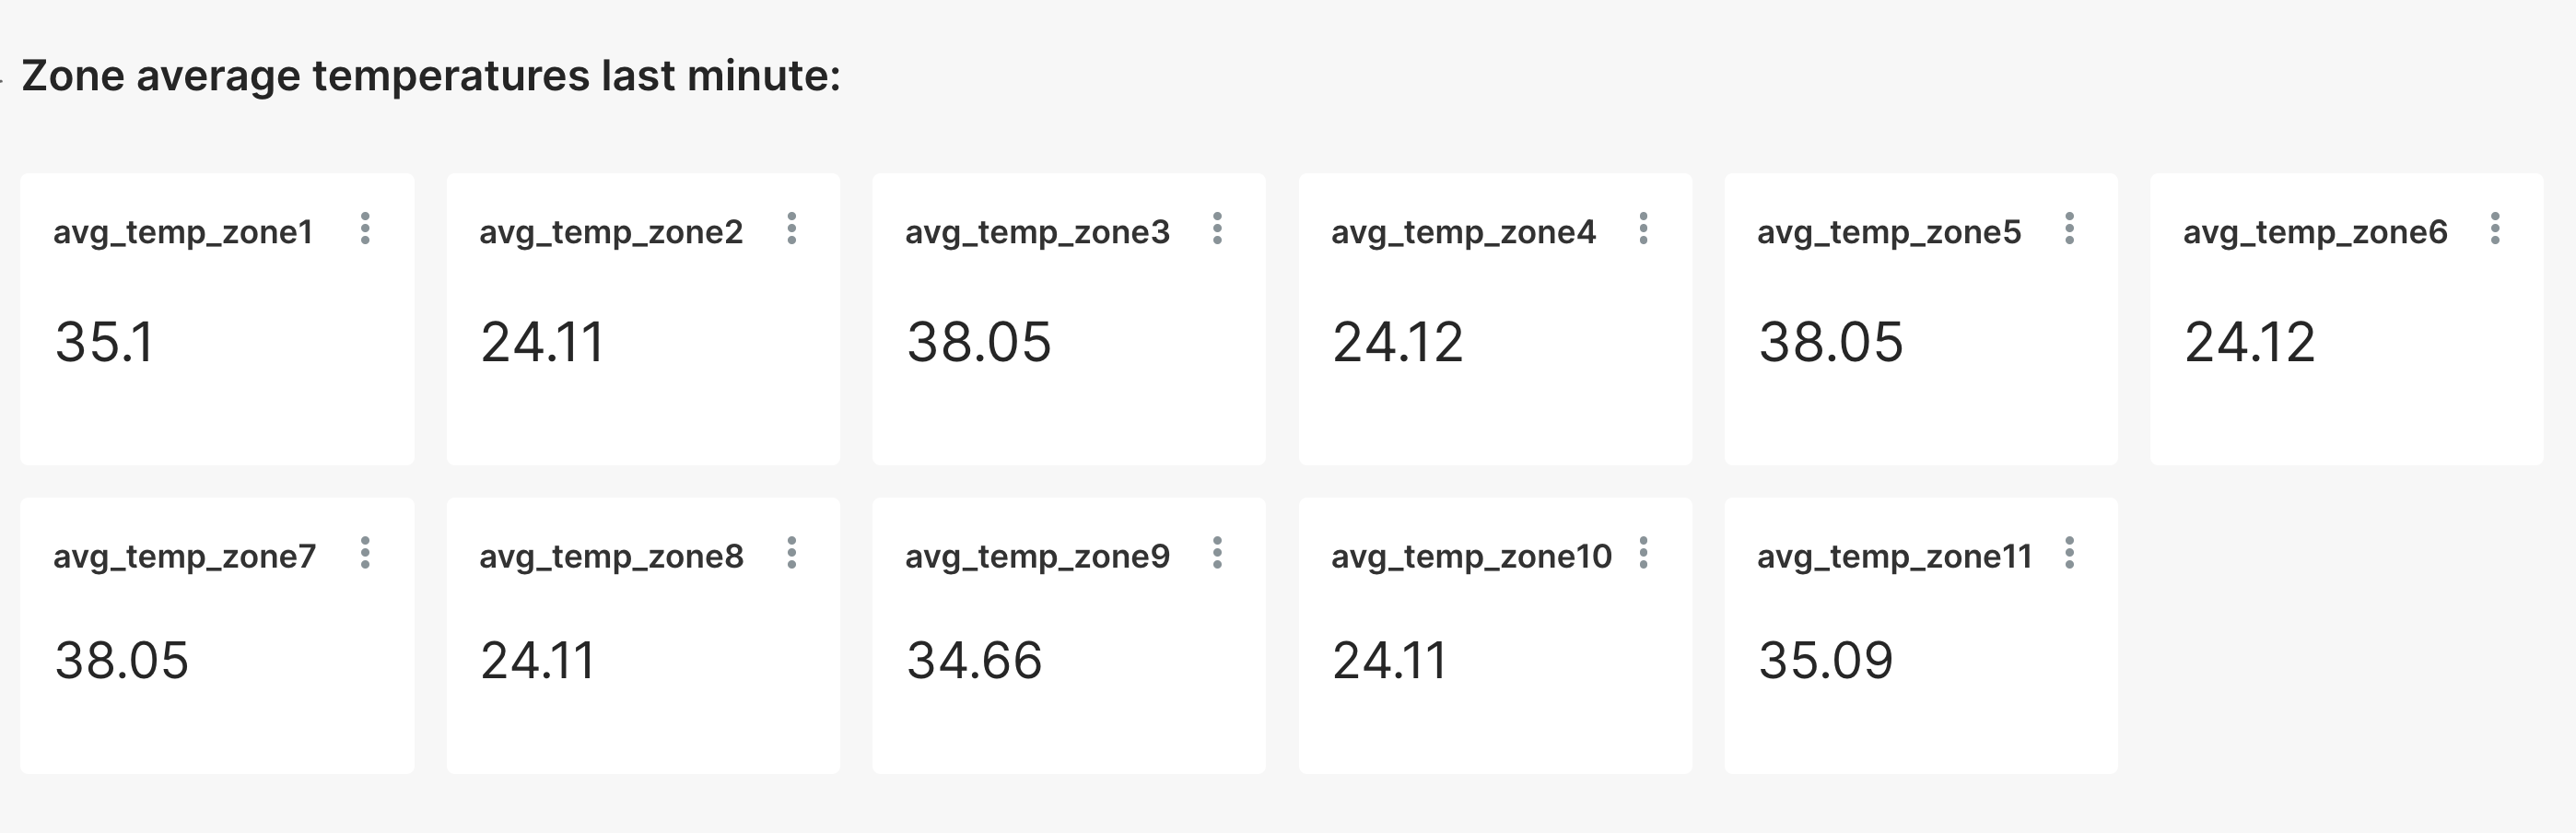
\includegraphics[width=0.9\linewidth]{figures/temp_section.png}
\captionof{figure}{Секция температур.}
\end{figure}
}

\item {\textbf{Секция Энергопотребления.} (Рис. 2). Эта секция визуализирует энергопотребление в ЦОД и состоит из двух графиков. Первый отвечает за общее энергопотребление ЦОД, а второй отображает энергопотребление системы охлаждения. График строится на данных за последний день, интервал наблюдений - 30 минут.

\begin{figure}[hbt!]
\centering
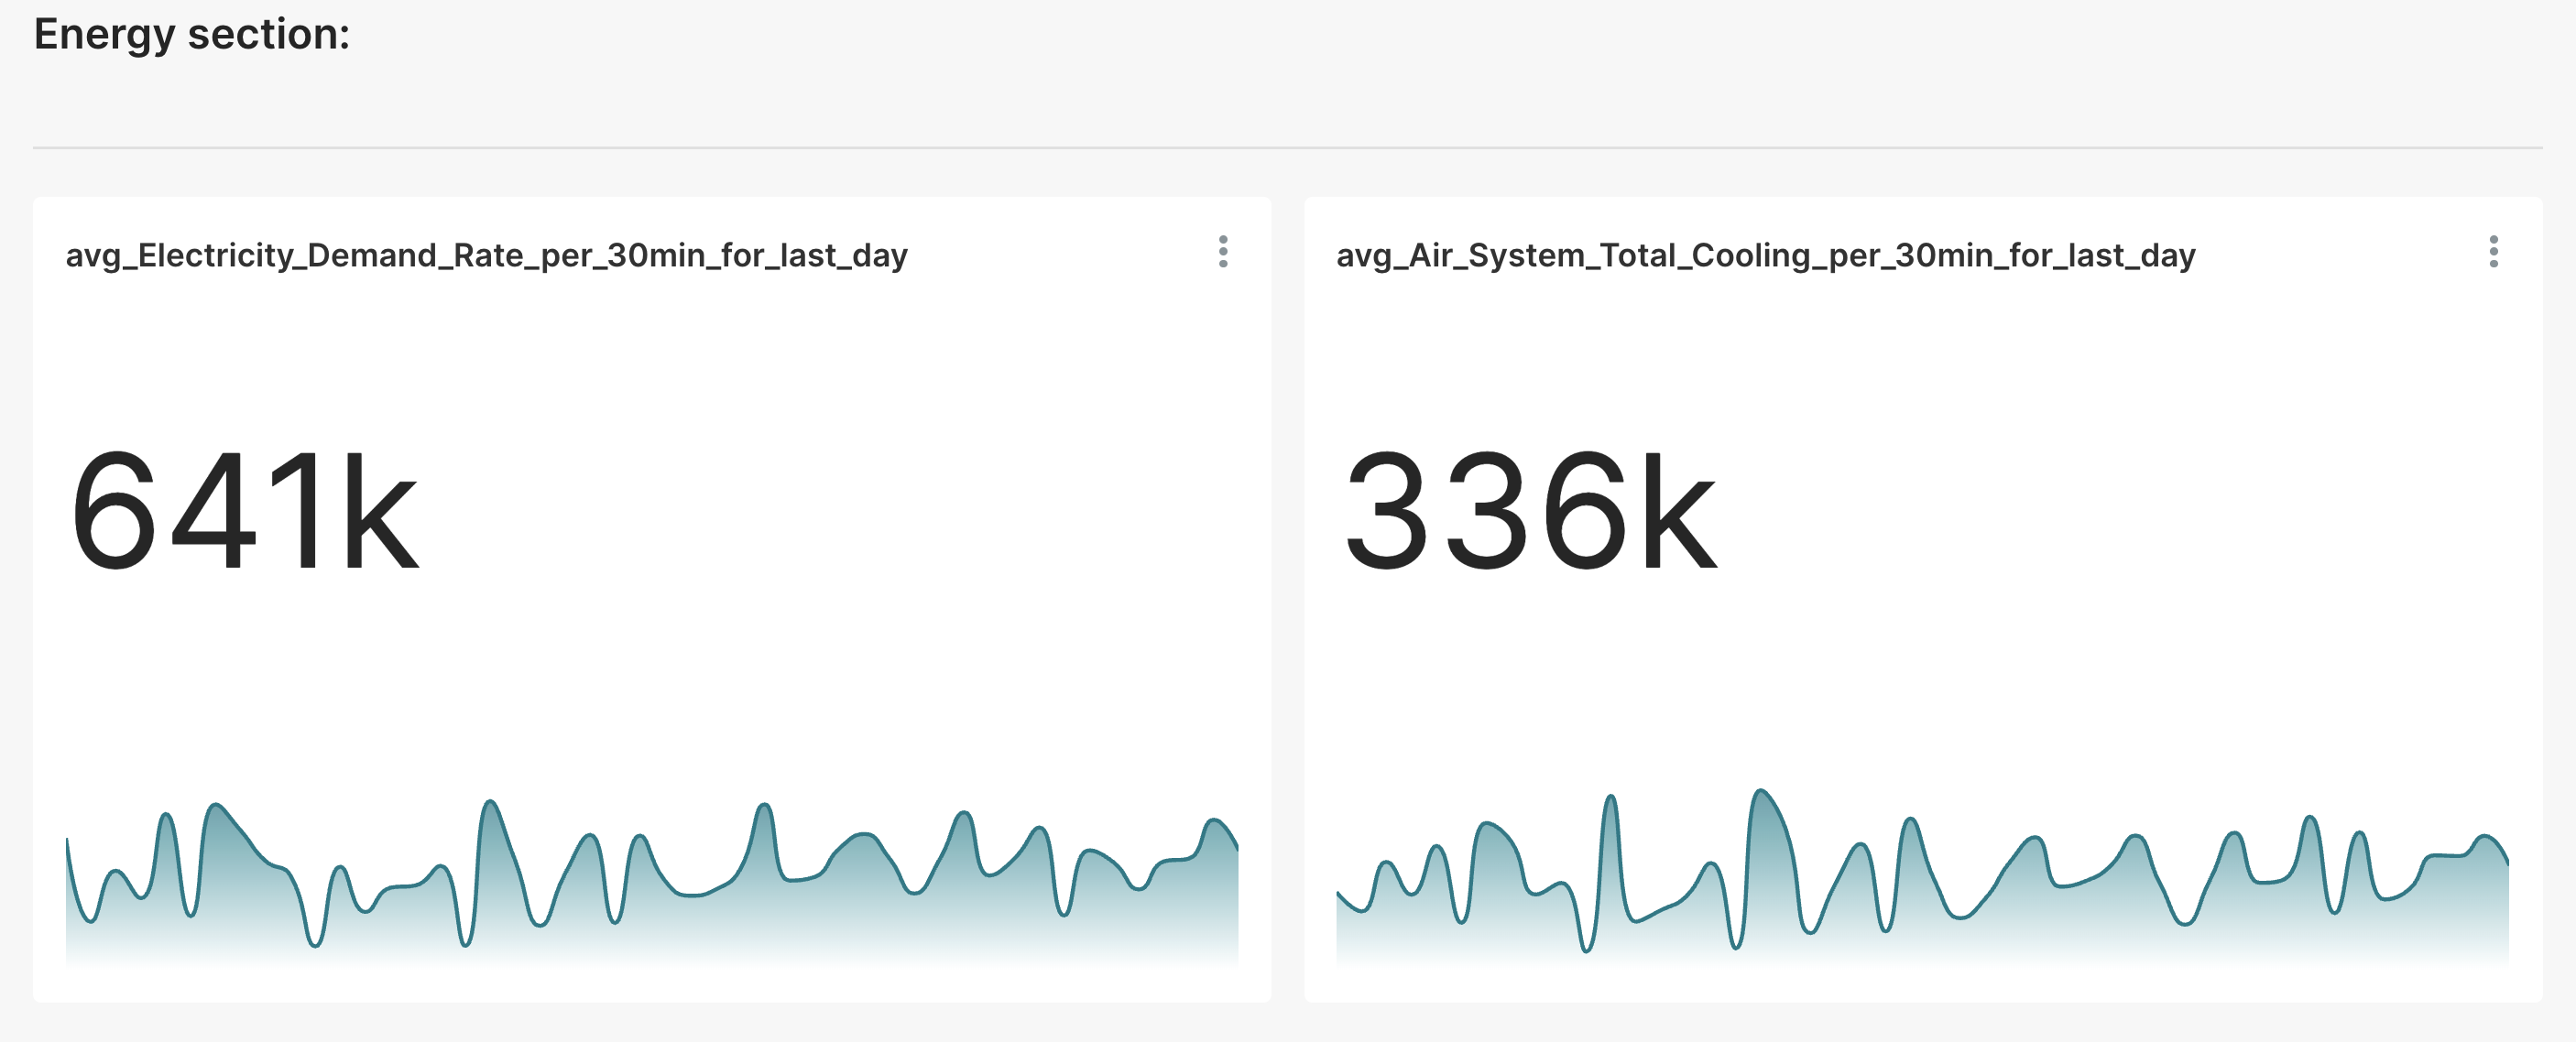
\includegraphics[width=0.9\linewidth]{figures/energy_section.png}
\captionof{figure}{Секция энергопотребления.}
\end{figure}
}

\item {\textbf{Секция Влажности.} (Рис. 3). В этой секции пользователь видит графики влажности первой центральной и последней зонах ЦОД.

\begin{figure}[hbt!]
\centering
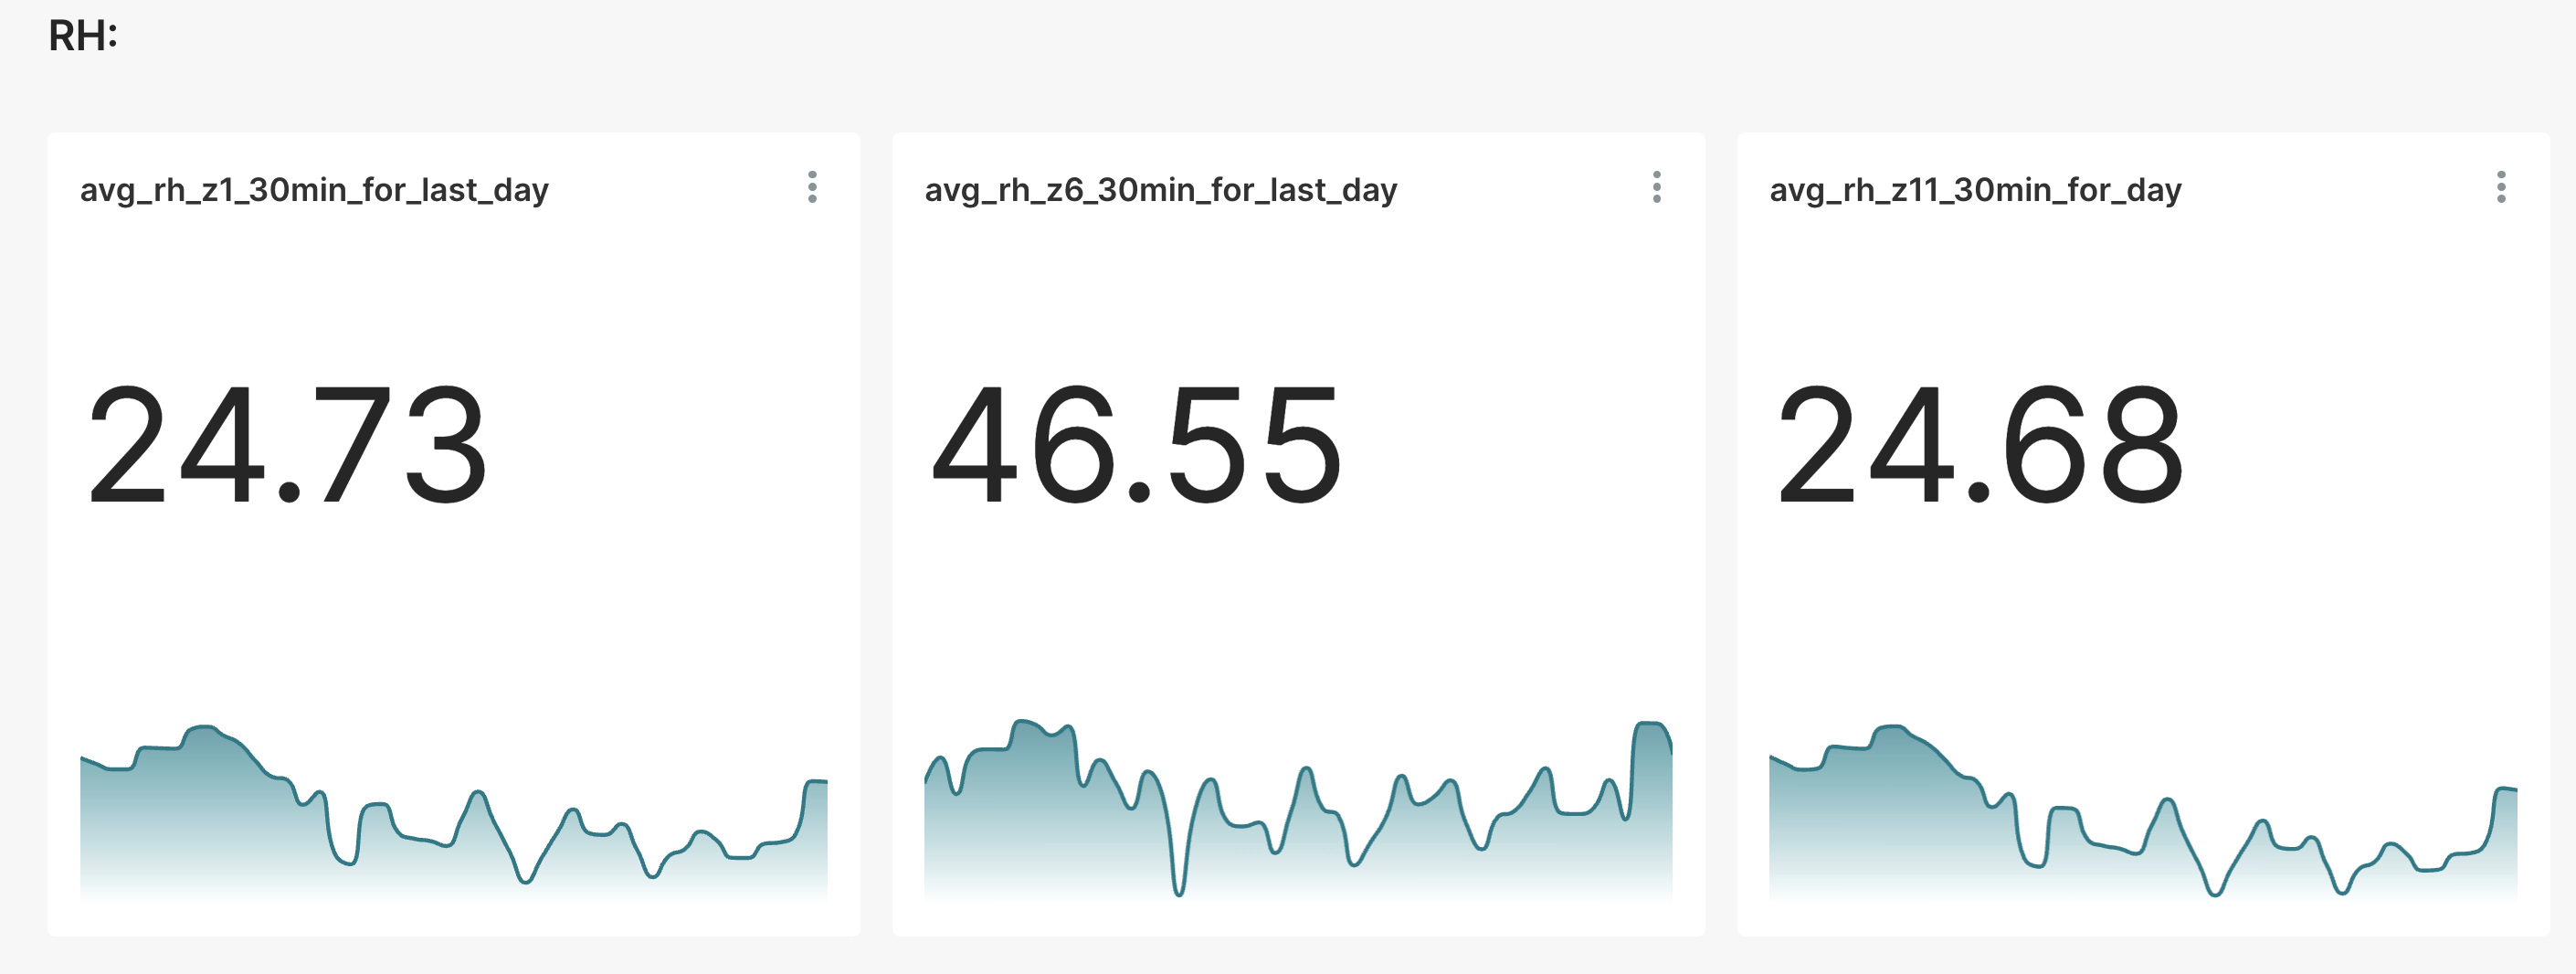
\includegraphics[width=0.9\linewidth]{figures/rh_section.png}
\captionof{figure}{Секция влажности.}
\end{figure}
}

\item {\textbf{Секция  CO\textsubscript{2}.} (Рис. 4). Здесь пользователь видит график уровня CO\textsubscript{2} (ppm.) для центарльной зоны ЦОД.

\begin{figure}[hbt!]
\centering
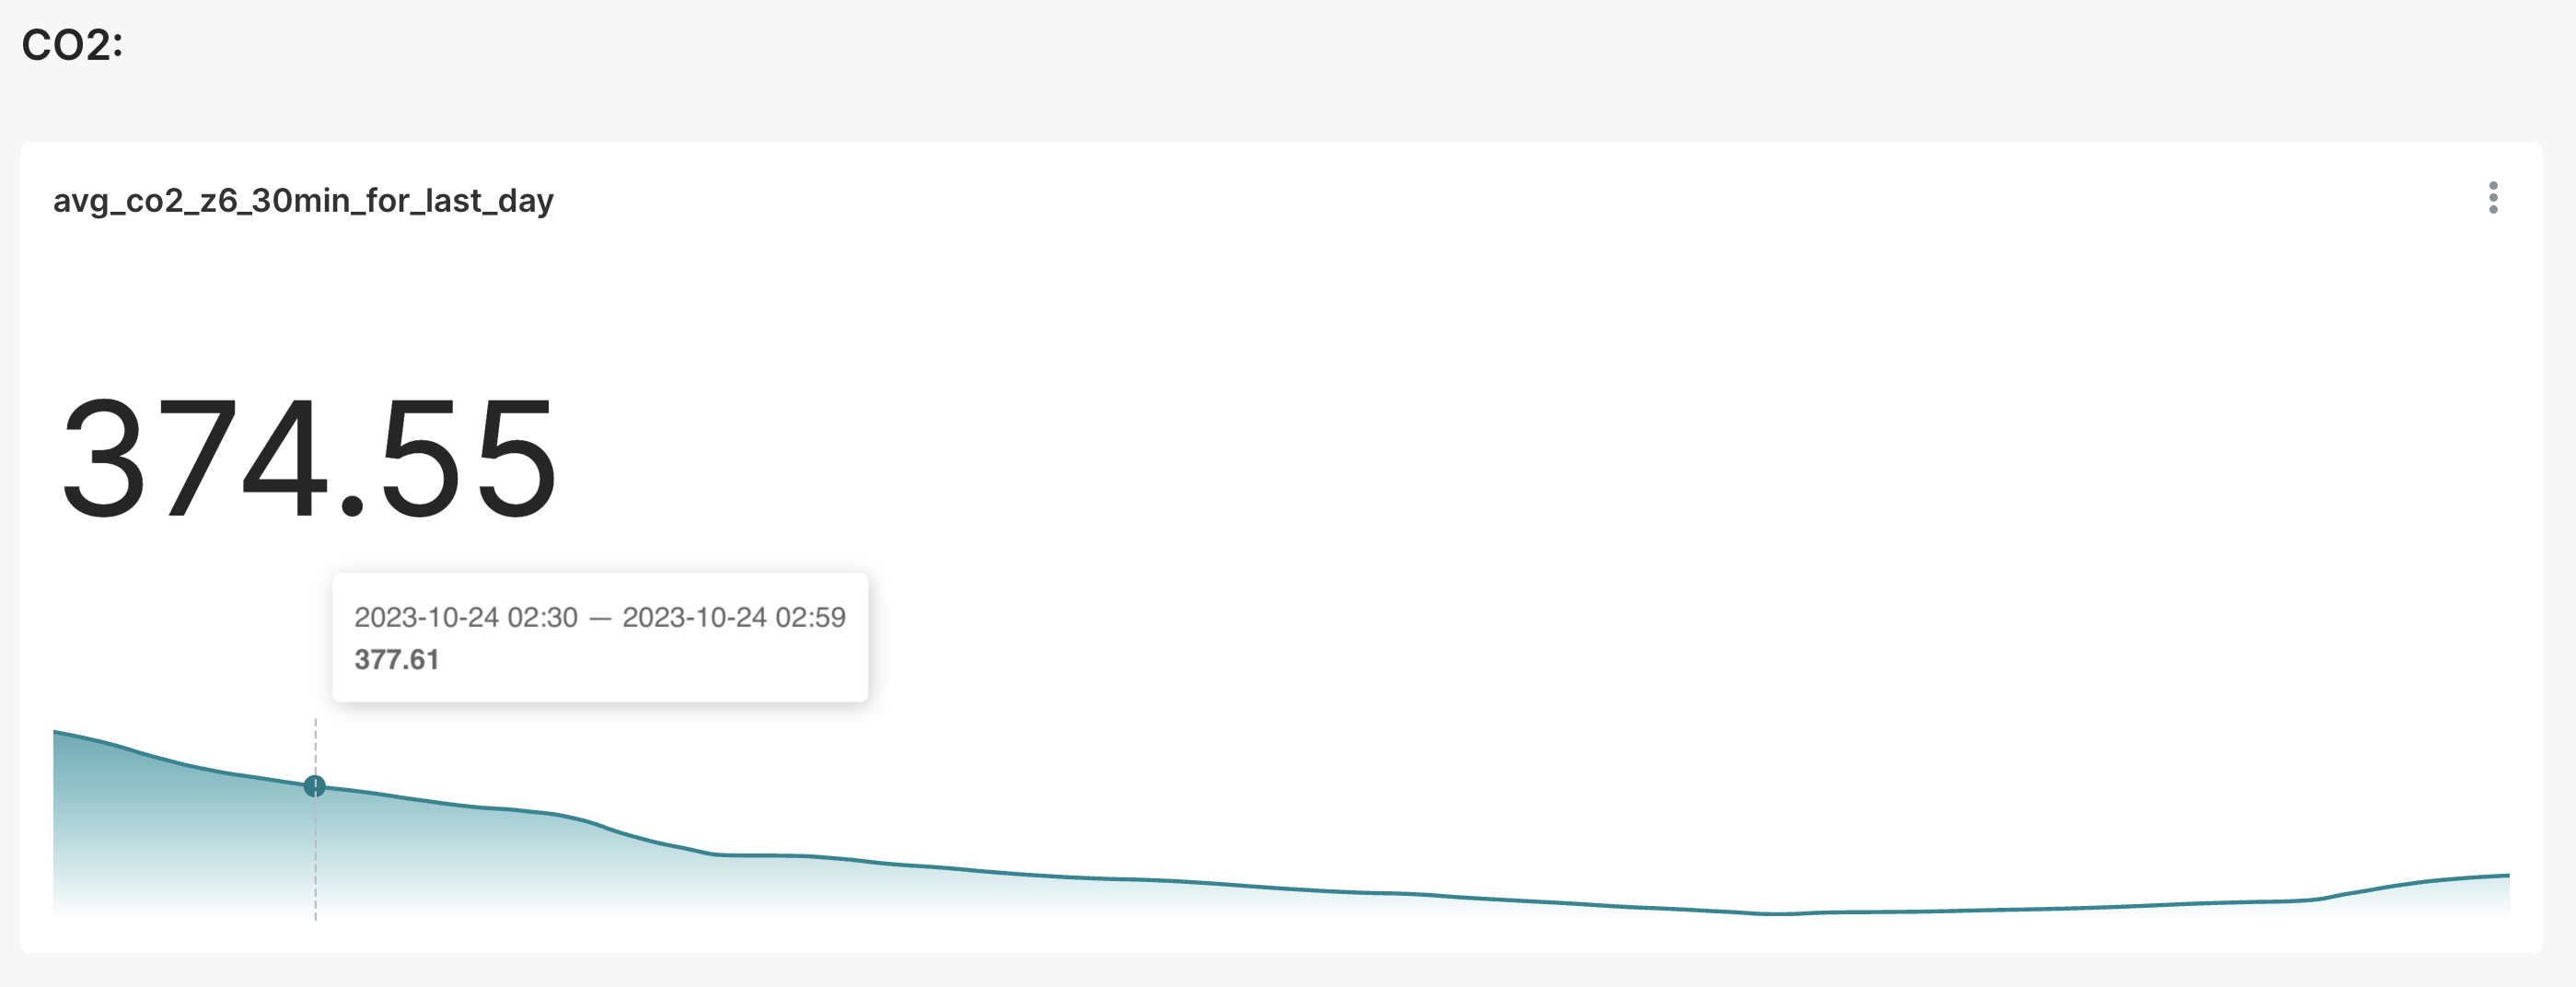
\includegraphics[width=0.9\linewidth]{figures/co2_section.png}
\captionof{figure}{Секция  CO\textsubscript{2}.}
\end{figure}

}

\end{itemize}



\end{document}